%%This is a very basic article template.
%%There is just one section and two subsections.
\documentclass[UTF8]{ctexart}
\title{第四章 SerDes接收端数据链路层设计}
\author{陈登}
\date{\today}

\bibliographystyle{plain}
\usepackage{graphicx}
\usepackage{float}
\usepackage{amsmath}
\usepackage{geometry}
\usepackage{fontspec}
\usepackage{algorithm}
\usepackage{algorithmicx}
\usepackage{algpseudocode}

\geometry{a4paper,centering,scale=0.9}
\usepackage[format=hang,font=small,textfont=it]{caption}
\usepackage[toc,page,title,titletoc,header]{appendix}
\usepackage[nottoc]{tocbibind}

\newcommand\kw{\textbf}

\begin{document}

\section{SerDes接收端数据链路层设计}

\subsection{8B/10B解码器设计}

根据JESD204B协议规定,SerDes接口为保证信内数据的直流平衡,并且为了便于时钟恢复,采用8B/10B码作为数据链路层的编码方式。
JESD204B中采用的8B/10B编解码部分主要参考IEEE802.3以太网协议中关于8B/10B的编解码部分。
但是由于应用环境的不同,JESD204B协议的8B/10B编解码方式同以太网相比略有不同。

\subsubsection{协议分析}

以太网协议提供了完整的编码表,也可以看作为解码表,这几张表格的正确性毋庸置疑,是最值得参考的资料。
表中将总共268种的编码情况全部列出,可以作为校验编码正确性的基准值。

在数字编码中有一个重要的概念,叫做极性\footnote{RD,即Running Disparity}。
极性是指一组编码中0的个数和1的个数之差,在一定长度的编码情况下,可以理解为0或1的个数。
比如说3B/4B编码中,在4B编码结果中,若1的个数多余0的个数则称为正极性,反之称为负极性,二者相同则称为平衡。
事实上,在具体的数据字编码中,不会出现编码结果0的个数多余1的个数三个或以上.
若编码中1的个数减去0的个数记,无论6B或者4B的编码结果只会为-2,0,2,相对应与负极性、平衡和正极性。

以太网协议建议,将一个码组的极性分为三部分,第一是上一码组计算后得出的极性,第二是编码后6B部分的极性,第三是编码后4B部分的极性。
而最后得到的4B部分的极性将作为这一组码的极性用于接下来码组的计算。
极性运算的基本结构:$last\_code\_group\_RD \to 6B\_sub\_block \to 6B\_RD \to 4B\_sub\_block \to 4B\_RD(new\_last\_code\_group\_RD)$。

每个sub-block的判断可用以下伪代码表示(6B和4B略有不同):

\begin{tabbing}
\qquad\=\kw{if} $000111$ or $0011$ or $1s>0s$ \\
      \>\qquad$6B\_RD=+;RD\_4B=+;$ \\
      \>\kw{else if} $111000$ or $1100$ or $1s<0s$ \\
      \>\qquad$6B\_RD=-;RD\_4B=-;$ \\
      \>\kw{else} \\
      \>\qquad$6B\_RD=last\_code\_group\_RD;$ \\
      \>\qquad$4B\_RD=6B\_RD;$ \\
      \>\kw{endif}
\end{tabbing}

最后是以太网协议中关于极性错误的处理,在协议附录中给出了一些接收当中的极性错误。
可以发现,极性错误是不能精确定位的,它的检测主要是通过接收机本地的极性和所接收到的极性不符所产生的错误。
但由于一系列的中性码并不会改变极性,前一码接收产生的错误可能因为一系列的中性码而直到几个码字后才能检测到。

在JESD204B协议中关于8B/10B编解码的规定,阅读接口协议的数据链路层内容,可以发现,在编解码器之前还有一级控制,主要是用来针对数据成帧结构中的lane、帧、多帧的校准、同步和错误控制,而控制的依据就是解码器中获得的控制字。

在JESD204B协议中只用到了8B/10B所用控制字的5个,这将简化控制字的解码复杂度,控制字分别如下:

\begin{description}
  \item[K.29.0] 即D,表示多帧的开始。
  \item[K.28.3] 即A,表示Lane校准,一般在多帧最后出现。
  \item[K.28.4] 即Q,表示Link设置数据的开始,在他之后跟一系列设置数据,配置Link,他也是ILAS\footnote{Initial Lane Alignment Sequence}的组成部分。
  \item[K.28.7] 即K,表示Group同步,可以说是链接开头最重要的部分,用来保持同步,是CGS\footnote{Code Group Synchronization}的重要控制字。
  \item[K.28.7] 即F,表示帧校准,一般表示一帧结束。
\end{description}

JESD204B协议还规定了三种重要的解码错误,这些在解码器级别的错误是属于不太严重的错误,有可能经常发生,在错误并不严重的情况下并不需要进行重同步,但是需要上报给错误处理部分,供应用层决定如何处理。

错误包括以下三种:

\begin{description}
  \item[Not-in-table Error] 这种错误意味着接收到的码字在任何极性情况下都不存在于码表中,就是一些非法的码字。对于这些码字,协议规定接收端需要重复之前收到的最新的没有错误的帧。
  \item[Running Disparity Error] 这种错误就是上文提到的极性错误,协议规定解码器要根据收到的数据和极性直接解码。由于在检测到极性错误时,可能产生错误的不是这个码字,这样的处理方式也比较合理。
  \item[Unexpected Control Character] 这种错误就是指未出现在指定位置的控制字,这一错误的具体处理需要由lane/帧监测部分来决定,属于接下来层级的处理,解码器并无法判断出这一错误。
\end{description}

\subsubsection{解码思路}

具体逻辑框图如图\ref{fig:8b10b_decoder_diagram}所示。

\begin{figure}[H]
\centering
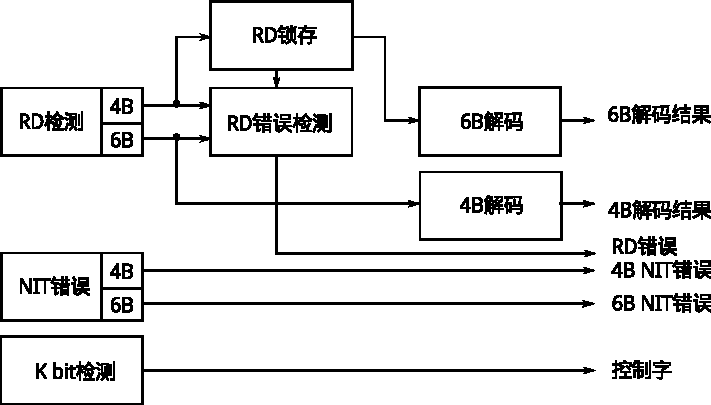
\includegraphics[width=14cm]{./img/8b10b_decoder_diagram.pdf}
\caption{8B/10B解码器系统框图}
\label{fig:8b10b_decoder_diagram}
\end{figure}

通过对现有论文编解码方式的理解分析,可以发现编码的方式比较多样,但解码仍主要停留在通过逻辑的方式。
在\cite{zhaoyh2003}、\cite{hecf2005}和\cite{Widmer1983}中采用的是纯逻辑解码方式;在\cite{wenl2007}和\cite{Actel1998}这两篇文章中采用的是多路选择器的方式。

在现有文章的解码中,极性仅作为差错检测,这是一种对信号资源的浪费,如果通过极性来进行解码,可以更好的利用现有的码表。
对于已知码组的极性信息,可以得出下一组码可能的编码情况,这时就可以通过取反操作来压缩解码表的大小,更快的处理解码操作。
例如,已知前一组码字的极性信息为$RD+$,则可以推测出接下来的$6B$数据的极性信息只有可能为$RD-$或者均衡两种可能。
因此只需要处理一种极性的码字就可以完成对整个编码的解码,复杂度变为原来的一半。

对于数据字而言,在获知当前$RD$状态的前提下,解码就分为两种情况。
一种是相反的极性,还有一种是均衡的极性。
对于相反的极性而言,不需要对另一种极性解码,整张解码用表就可以缩小一半,一方面节约了芯片面积额,一方面提高了解码效率。
对于均衡极性而言,由\cite{Widmer1983}中编码原理分析可知,对于均衡码的解码其实非常简便,只需要输出其低$5$或$3$位。
因此,只需要设计一个均衡码判断电路,就可以快速选择是否通过解码逻辑极性解码。

对于控制字而言,由\cite{Actel1998}中提到的控制信息检测可以发现,通过$RD$和固定位置的比特就可以区分该码字是否为控制字,并且确定是哪一类控制字($K.28.x$还是$K.23.7$、$K.27.7$、$K.29.7$、$K.30.7$)。
在分析编码可知,控制字的$3B$或$5B$部分的编码规则同数据字是相同的。那么就可以“借用”数据字的解码部分来对控制字部分解码,准确输出控制码字。
其中包括了均衡和非均衡的情况,处理逻辑同数据字,唯一不同的就是控制字状态标记是否拉高。

最后对于解码模块的考虑,一般情况下都是采用的是verilog语言的case逻辑,但是对于高效的电路来说要尽量避免对语言原生性能的依赖。
通过逻辑化简的方法对更小的码表进行化简,这样的得到表达式速度更快,并且面积较小。

\subsubsection{第一级,预处理级}

预处理级系统框图如图\ref{fig:8b10b_preprocess_model}所示。

\begin{figure}[H]
\centering
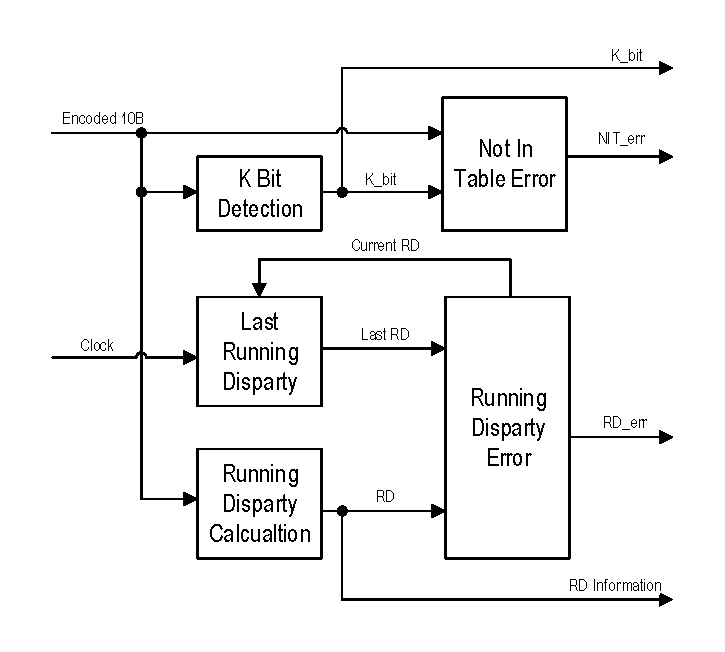
\includegraphics[width=14cm]{./img/8b10b_preprocess_model.pdf}
\caption{8B/10B解码器预处理级框图}
\label{fig:8b10b_preprocess_model}
\end{figure}

\paragraph{K Bit检测}

根据输入完整的$10B$数据判断是否为控制信号。
有以下伪代码:

\begin{tabbing}
\qquad\=\kw{if} $iedc==1111|0000$ \\
      \>\qquad$K.28.x=1;K.x.7=0;$ \\
      \>\kw{else if} $jhgfie==010111|101000$ \\
      \>\qquad$K.28.x=0;K.x.7=1;$ \\
      \>\kw{else} \\
      \>\qquad$K.28.x=0;K.x.7=0;$ \\
      \>\kw{endif}
\end{tabbing}

本设计中的8B/10B编码,只采用了6B部分为K.28的控制字。
由完整检测逻辑可以得出,只需要检测6B部分的cdei位是否为0000或者1111,就能判断出结果。
所以判断控制字本设计可以采用最简单的逻辑表达式:

$$K\_bit = (c \& d \& e \& i)\quad|\quad~(c | d | e | i)$$

\paragraph{$6B$和$4B$平衡检测}

就是对给出的并行数据,分别输出$6B$和$4B$是否平衡,平衡即指0和1的数量是否相同。
有以下伪代码\footnote{其中$RL$表示游程长度计算,即$1$的个数。下同。}:

\begin{tabbing}
\qquad\=\kw{if} $RL(6B)==3$ \\
      \>\qquad$Balance\_6B=1;$ \\
      \>\kw{else} \\
      \>\qquad$Balance\_6B=0;$ \\
      \>\kw{endif}
\end{tabbing}

\begin{tabbing}
\qquad\=\kw{if} $RL(4B)==2$ \\
      \>\qquad$Balance\_4B=1;$ \\
      \>\kw{else} \\
      \>\qquad$Balance\_4B=0;$ \\
      \>\kw{endif}
\end{tabbing}

\paragraph{RD信息检测}

RD信息检测主要指分别计算6B和4B部分的极性,每一部分又分别有两个输出,$RD-$和$RD+$。
因为每一组码字的极性一共存在三种可能,即正、负和平衡,不属于负和正的码字,既为平衡,平衡的判断也可由上文中的伪代码确定。
这些重要的信息主要用于极性错误检测和解码。
通过对合法码字的真值表进行化简,可以得到快速RD极性检测模块,准确输出正确码字RD的负和正信号。

最终模块输出4个信号,即RD\_6B\_pos、RD\_6B\_neg、RD\_4B\_pos、RD\_4B\_neg。

\paragraph{NIT错误检测}

Not-In-Table Error的检测也分为4B和6B两部分。

6B部分的错误码字一共为14种,如表\ref{tab:tab_6B_NIT_err},参考\cite{Widmer1983}一文的方法可以分为两类,既考虑abcd全为0或全为1的情况和abcd有且仅有1个1或仅有1个0的情况。
前者直接可以判断该码字为错误码字,后者再观察ef是否全为0或全为1,也可判断码字是否错误。

4B部分的错误码字相对较为复杂,考虑到K.28中只有5个控制字是合法的,所以要对余下的码字报错。
4B部分报错情况如表\ref{tab:tab_4B_NIT_err}所示。

\begin{table}[H]
\begin{minipage}[t]{.5\textwidth}
\centering
\caption{6B码字错误情况}
\label{tab:tab_6B_NIT_err}
\begin{tabular}{|c|r|r|r|}
\hline
	abcdei	&	abcdei	\\
\hline
	000000	&	111111	\\
	000001	&	111110	\\
	000010	&	111101	\\
	000100	&	111011	\\
	001000	&	110111	\\
	010000	&	101111	\\
	100000	&	011111	\\
\hline
\end{tabular}
\end{minipage}
\begin{minipage}[t]{.5\textwidth}
\centering
\caption{4B码字错误情况}
\label{tab:tab_4B_NIT_err}
\begin{tabular}{|c|r|r|r|}
\hline
	abcdei	&	hgfj	\\
\hline
	xxxxxx	&	0000	\\
			&	1111	\\
\hline
	001111	&	0101	\\
			&	1001	\\
			&	0110	\\
\hline
	110000	&	1010	\\
			&	1001	\\
			&	0110	\\
\hline
\end{tabular}
\end{minipage}
\end{table}

极性错误检测部分负责检测关于极性的错误,主要就是指不能出现连续相同的极性变化。
例如之前一个码字的RD为RD-,则接下来收到的6B编码的RD必须为均衡或者是RD+,这样就保证了信道上码字的均衡。
极性检测实际上考虑的是三个部分的信息,可以细化为五个信号,包括上一个码字的极性,当前码字6B部分的RD+或RD-,当前码字4B部分的RD+或RD-。
极性错误的监测并不能精确定位,因为均衡的码字是无法判断出是否有错的,只有当数据扩散到非均衡位置时才能判断出错误。
由于正确的检测需要保存上一码字的极性信息,所以极性错误检测还负责解码器极性的刷新。
检测可以通过极性信息计算模块提供的信号进行判断,并将得到新的极性存入寄存器,如表\ref{tab:tab_RD_err}所示。

\begin{table}[H]
\centering
\caption{极性错误检测及新极性生成表}
\label{tab:tab_RD_err}
\begin{tabular}{|c|c|c|c|c|c|c|}
\hline
	last	&	6B+	&	6B-	&	4B+	&	4B-	&	err	&	new	\\
\hline
	0 	 	&	0 	&	0 	& 	0	&	0 	&	0 	&	0 	\\
	0 	 	&	0 	&	0 	& 	0	&	1 	&	1 	&	0 	\\
	0 	 	&	0 	&	0 	& 	1	&	0 	&	0 	&	1 	\\
	0 	 	&	0 	&	1 	& 	0	&	0 	&	1 	&	0 	\\
	0 	 	&	0 	&	1 	& 	0	&	1 	&	1 	&	0 	\\
	0 	 	&	0 	&	1 	& 	1	&	0 	&	1 	&	1 	\\
	0 	 	&	1 	&	0 	& 	0	&	0 	&	0 	&	1 	\\
	0 	 	&	1 	&	0 	& 	0	&	1 	&	0 	&	0 	\\
	0 	 	&	1 	&	0 	& 	1	&	0 	&	1 	&	1 	\\
	1 	 	&	0 	&	0 	& 	0	&	0 	&	0 	&	1 	\\
	1 	 	&	0 	&	0 	& 	0	&	1 	&	0 	&	0 	\\
	1 	 	&	0 	&	0 	& 	1	&	0 	&	1 	&	1 	\\
	1 	 	&	0 	&	1 	& 	0	&	0 	&	0 	&	0 	\\
	1 	 	&	0 	&	1 	& 	0	&	1 	&	1 	&	0 	\\
	1 	 	&	0 	&	1 	& 	1	&	0 	&	0 	&	1 	\\
	1 	 	&	1 	&	0 	& 	0	&	0 	&	1 	&	1 	\\
	1 	 	&	1 	&	0 	& 	0	&	1 	&	1 	&	0 	\\
	1 	 	&	1 	&	0 	& 	1	&	0 	&	1 	&	1 	\\
\hline
\end{tabular}
\end{table}

根据此表化简逻辑表达式即可得到准确的极性错误和本码字的极性情况。
也可以采用有限状态机的方法进行判断,通过几个固定的状态转换进行极性的判断和存储了\cite{AlKafi2013}。
极性状态转移图如图\ref{fig:8b10b_running_disparity_status}所示。

\begin{figure}[H]
\centering
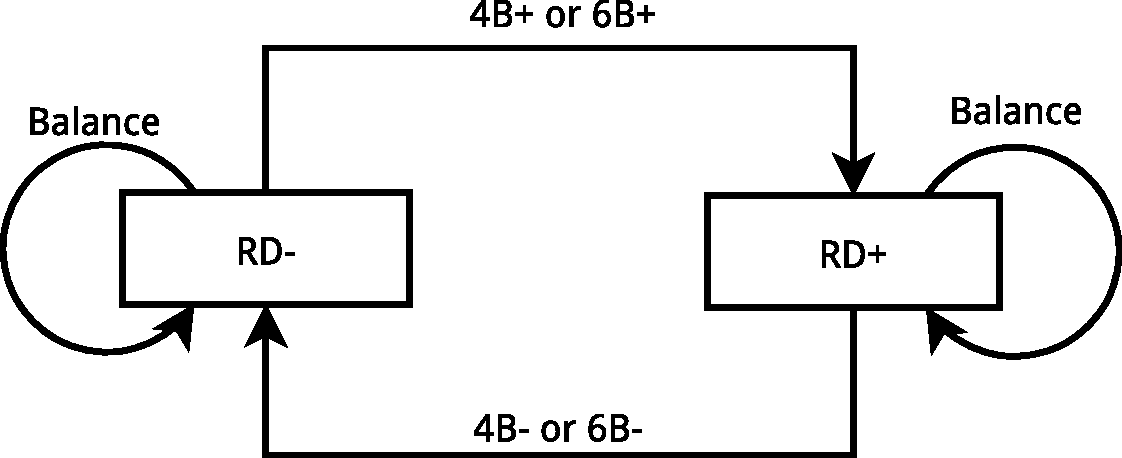
\includegraphics[width=10cm]{./img/8b10b_running_disparity_status.pdf}
\caption{8B/10B Running Disparity状态转移图}
\label{fig:8b10b_running_disparity_status}
\end{figure}

\subsubsection{第二级,解码级}

解码级系统框图如图\ref{fig:8b10b_decoder_model}所示。

\begin{figure}[H]
\centering
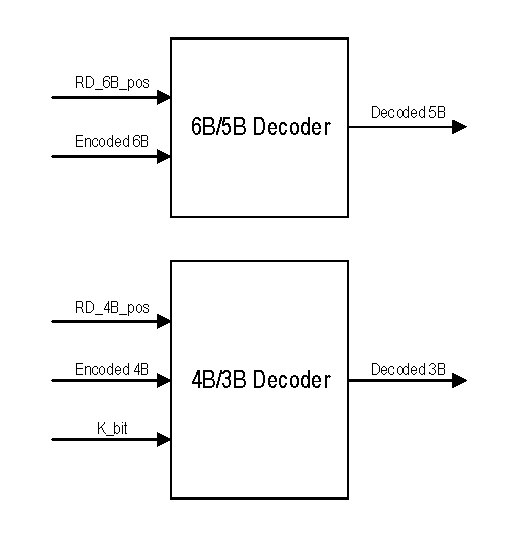
\includegraphics[width=10cm]{./img/8b10b_decoder_model.pdf}
\caption{8B/10B解码器解码级框图}
\label{fig:8b10b_decoder_model}
\end{figure}

解码输入的第一步就是根据极性情况,对输入码字进行反转。
根据8B/10B原理,对于相同的原始码字编码,在不同极性情况下的变化就是互为反码。
所以在知道具体码字的极性信息时对其进行反转就可以准确的得到同极性下的编码,使之后的解码器只需要处理一种极性。
具体的反转判断伪代码如下:

\begin{tabbing}
\qquad\=\kw{if} $RD==RD+$ \\
      \>\qquad$6B=6B;$ \\
      \>\kw{else} \\
      \>\qquad$6B=!6B;$ \\
      \>\kw{endif}
\end{tabbing}

\begin{tabbing}
\qquad\=$RD\_6=RD|Balance\_6B$ \\
      \>\kw{if} $RD\_6==RD+$ \\
      \>\qquad$4B=4B;$ \\
      \>\kw{else} \\
      \>\qquad$4B=!4B;$ \\
      \>\kw{endif}
\end{tabbing}

$6B/5B$和$4B/3B$解码部分,主要根据解码表对输入码字解码。
解码表中存的查找项均为极性为正时的解码,根据输入输出解码结果,5B/6B解码部分解码表如表\ref{tab:tab_6B_tab}所示,3B/4B解码部分解码表如表\ref{tab:tab_4B_tab}所示。

需要特别注意的是3B/4B解码部分,不同于5B/6B解码,3B/4B解码还需要考虑控制字的信息。
这是因为对于特定的控制字K.28来说,为了避免整个10B编码偶然的出现连续5个0或1,解码器就要根据情况来选择不同的3B编码。
在解码过程中要着重考虑到这一点,为此增加了K位作为解码输入条件之一,K位即表示控制位,由预处理级的控制字检测电路产生。
通过化简增加信息后的真值表,得到表达式用以解码。

最后需要考虑的是均衡码字的情况,这种情况可以由之前的极性信息直接推断出来,这时候解码器需要做的就是输出相应解码部分的低位。

不同于\cite{Actel1998}文中所描述的CASE方法,也不同于\cite{Widmer1983}中的纯逻辑方法。
本设计引入了各个模块的$RD+$信息,在读入数据之前先根据RD\_pos信息对码字进行反转。
这样,在解码时只要考虑$RD$为$RD-$和平衡的情况。
对于6B解码表由原来的48种情况减少为34种(如表\ref{tab:tab_6B_tab}所示);对于4B解码表,由于其解码需要考虑K Bit的情况,由原来的28种情况减少为16种(如表\ref{tab:tab_4B_tab}所示)。
并且由于快速的极性信息计算,使得解码模块能够更快的进行解码,缩短了解码所需时间。
最后通过逻辑化简的方法对更小的码表进行化简,这样的得到表达式速度更快,并且面积较小。

\begin{table}[H]
\begin{minipage}[t]{.5\textwidth}
\centering
\caption{6B解码表}
\label{tab:tab_6B_tab}
\begin{tabular}{|c|c|c|c|}
\hline
	abcdei	&	EDCBA	&	abcdei	&	EDCBA	\\
\hline
	000011	&	11100	&	011001	&	11001	\\
	000101	&	01111	&	011010	&	11010	\\
	000110	&	00000	&	011100	&	11100	\\
	000111	&	00111	&	100001	&	11110 	\\
	001001	&	10000	&	100010	&	11101 	\\
	001010	&	11111	&	100011	&	00011 	\\
	001011	&	01011	&	100100	&	11011 	\\
	001100	&	11000	&	100101	&	00101 	\\
	001101	&	01101	&	100110	&	00110 	\\
	001110	&	01110	&	101000	&	10111 	\\
	010001	&	00001	&	101001	&	01001 	\\
	010010	&	00010	&	101010	&	01010 	\\
	010011	&	10011	&	101100	&	01100 	\\
	010100	&	00100	&	110001	&	10001 	\\
	010101	&	10101	&	110010	&	10010 	\\
	010110	&	10110	&	110100	&	10100 	\\
	011000	&	01000	&	111000	&	00111 	\\
\hline
\end{tabular}
\end{minipage}
\begin{minipage}[t]{.5\textwidth}
\centering
\caption{4B解码表}
\label{tab:tab_4B_tab}
\begin{tabular}{|c|c|c|}
\hline
	K	&	hgfj	&	HGF	\\
\hline
	0	&	0001	&	111	\\
	0	&	0010	&	000	\\
	0	&	0011	&	011	\\
	0	&	0100	&	100	\\
	0	&	0101	&	101	\\
	0	&	0110	&	110	\\
	0	&	1000	&	111	\\
	0	&	1001	&	001	\\
	0	&	1010	&	010	\\
	0	&	1100	&	011	\\
	1	&	0001	&	111	\\
	1	&	0010	&	000	\\
	1	&	0011	&	011	\\
	1	&	0100	&	100	\\
	1	&	1010	&	101	\\
	1	&	1100	&	011	\\
\hline
\end{tabular}
\end{minipage}
\end{table}

\subsection{解扰器设计}

JESD204的发送端和接收端设备都需要支持加扰传输的数据流。
并且每一对lane都要包含加扰器和解扰器。
加扰器和解扰器的位置位于数据链路层和传输层之间,也就是位于8B/10B解码器之后进行解扰,加扰后进行编码。
所以加扰操作主要是针对数据进行的,不涉及链路上的控制字符。
对一个link启动加解扰意味着在link两端启动所有lane的加扰器和解扰器。
但采用混合模式,只对一个link中的固定几条lane启动加解扰器是不允许的。

加扰的主要目的是避免频谱出现过大的峰值,这就意味着过多的帧到帧之间重复数据传输。
在一个敏感的系统中,频谱的峰值会引起电磁不兼容或者互相干扰的问题。
过多相同帧也会引起基于编码的直流偏置。
另一个加扰的好处就是使传输信道的频谱和数据区分开,这样接口上可能的频率选择效应就不会影响到数据的独立性。

\subsubsection{协议分析}

每一种扰码都有相对应的符合实际传输需求的扰码多项式,作为加扰和解扰的依据。
JESD204B协议规定的扰码多项式如式\ref{eq:scrambler_polnomial}所示。

\begin{equation}
\label{eq:scrambler_polnomial}
1+x^{14}+x^{15}
\end{equation}

可见这个加扰多项式的周期长达32767位,足以符合敏感电磁系统频谱的要求。
并且他允许解扰器在接收到2个octet数据后达成自同步。

加扰器和解扰器的根据它们的串行实现,一帧一阵的处理发送和接受的数据。
一帧中最左边的位首先被转换,具体的转换顺序如图\ref{fig:serial_scrambling}所示。

\begin{figure}[H]
\centering
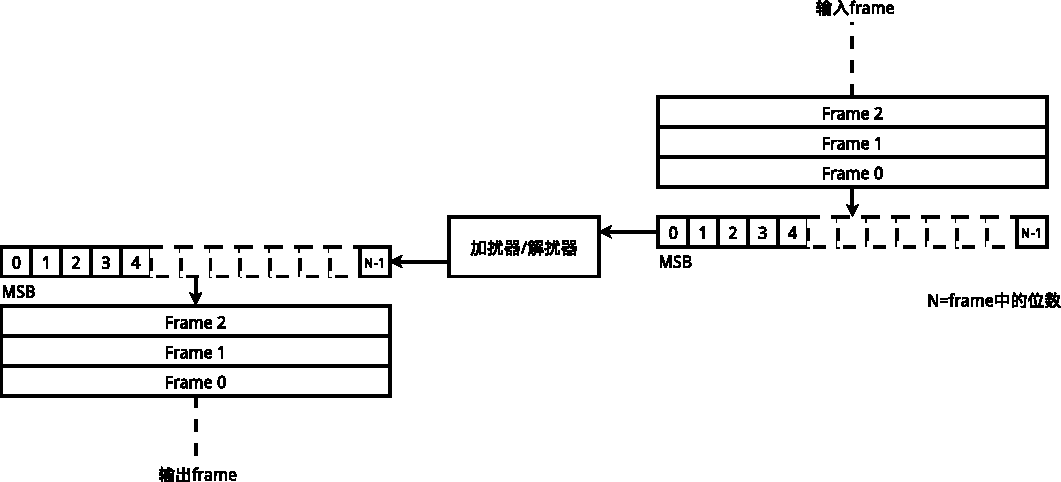
\includegraphics[width=18cm]{./img/serial_scrambling.pdf}
\caption{扰码帧传输顺序}
\label{fig:serial_scrambling}
\end{figure}

加扰器和解扰器要能够实现自同步,就是在没有额外初始信号的情况下,最终能够正确输出加扰编码。
针对JESD204B的协议规定的扰码多项式,可以得到解扰器串行实现的流程框图,如图所示。

加扰器串行更新函数如式\ref{eq:scrambled_serial_equation}所示。

\begin{equation}
\label{eq:scrambled_serial_equation}
S_{15} = D_{15} + S_1 + S_0
\end{equation}

加扰器并行更新函数如式\ref{eq:scrambled_parallel_equation}所示。

\begin{equation}
\label{eq:scrambled_parallel_equation}
\begin{cases}
	S_{31} = D_{31} + S_{17} + S_{16} \\
	S_{30} = D_{30} + S_{16} + S_{15} \\
	\dots							  \\
	S_{23} = D_{23} + S_{9} + S_{8}   \\
	S_{22} = D_{22} + S_{8} + S_{7}   \\
	\dots							  \\
	S_{17} = D_{17} + S_{3} + S_{2}   \\
	S_{16} = D_{16} + S_{2} + S_{1}   \\
\end{cases}
\end{equation}

解扰器串行更新函数如式\ref{eq:descrambled_serial_equation}所示。

\begin{equation}
\label{eq:descrambled_serial_equation}
D_{15} = S_{15} + S_1 + S_0
\end{equation}

解扰器并行更新函数如式\ref{eq:descrambled_parallel_equation}所示。

\begin{equation}
\label{eq:descrambled_parallel_equation}
\begin{cases}
	D_{31} = S_{31} + S_{17} + S_{16} \\
	D_{30} = S_{30} + S_{16} + S_{15} \\
	\dots							  \\
	D_{23} = S_{23} + S_{9} + S_{8}   \\
	D_{22} = S_{22} + S_{8} + S_{7}   \\
	\dots							  \\
	D_{17} = S_{17} + S_{3} + S_{2}   \\
	D_{16} = S_{16} + S_{2} + S_{1}   \\
\end{cases}
\end{equation}

其中,D表示为未加扰的原始数据位,S表示加扰状态位即加扰数据输出。

扰码的使能也是协议中重点规定的部分。
加扰只是针对用户数据,并不包括控制字信息,例如码群同步控制字符串和初始化帧对齐序列。
事实上,在传输中,前两个octet并不会全部进行加扰,因为发送端的加扰器也需要这两个octet作为初始化信息,才能正确进行之后的扰码输出。
但是两个octet中的最后一位需要根据第一位、第二位和最后一位自己,加扰得到一个新的加扰位进行传输,接下来的数据将需要进行正规的加扰。
在解扰端的状态寄存器跟踪上扰码同步前需要先接收两个octet的前15位作为初始化信息,之后才能根据第16位和之前接收到的第一第二位正确的输出解扰后数据。
为了避免在最初的两个octet处理时同正常的加扰区分开来,需要加解扰器有使能开关来切换是否进行解扰或者加扰。
在接收端,解扰器的输入端连接在8B/10B解码器的输出端,有一个使能开关决定数据是进行解扰还是直接通过。

所以,总体的加扰流控制图如图\ref{fig:scrambler_descrambler_implementation}所示。

\begin{figure}[H]
\centering
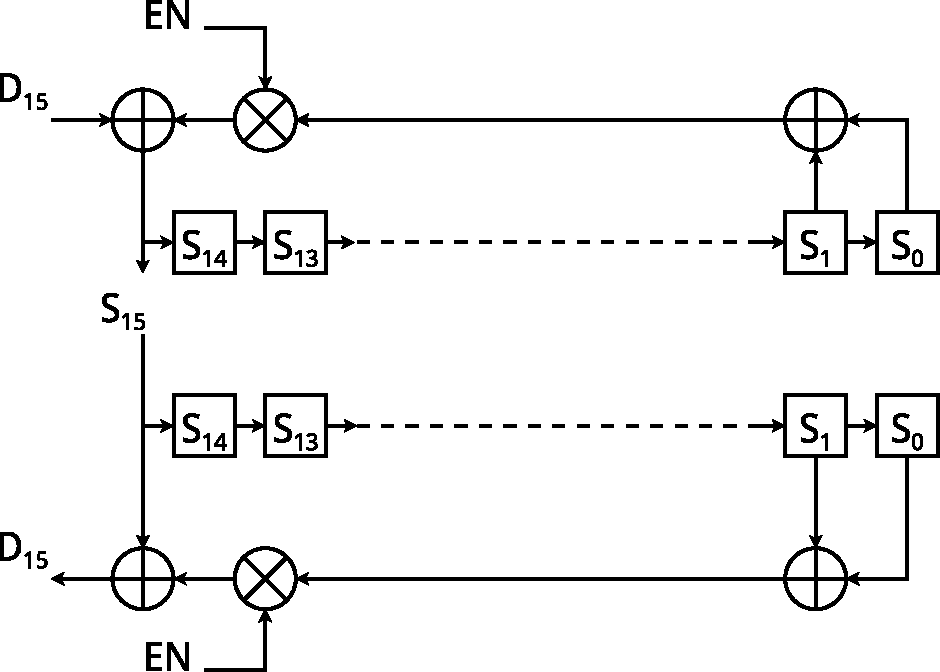
\includegraphics[width=18cm]{./img/scrambler_descrambler_implementation.pdf}
\caption{解扰器和加扰器实现流程框图}
\label{fig:scrambler_descrambler_implementation}
\end{figure}

最后需要考虑的是加解扰的初始状态问题。
同很多使用自同步的加扰器一样,当输入数据是重复的初始状态值时,将会产生重复的加扰输出。
这就失去了加扰的意义,使信号的波形产生较大的峰值,会导致借口的电磁串扰。
为了尽量避免重复输出,加扰器的初始状态必须设置为一个在传输层不太可能产生的octet。
推荐的初始值是高位8个1,余下各位为0,即111111110000000。

\subsubsection{解扰思路}

具体逻辑框图如图\ref{fig:scrambler_descrambler_parallel_implementation}所示。

\begin{figure}[H]
\centering
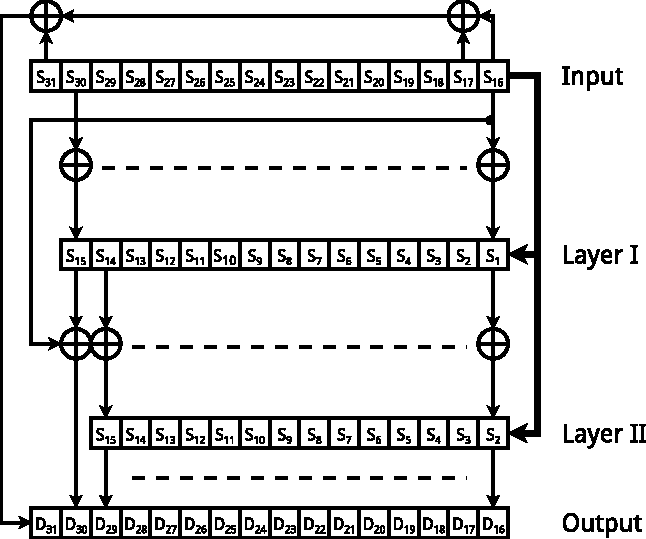
\includegraphics[width=18cm]{./img/scrambler_descrambler_parallel_implementation.pdf}
\caption{解扰器并行实现}
\label{fig:scrambler_descrambler_parallel_implementation}
\end{figure}

为了适应高速的处理环境,解扰器的尽量采用并行设计的思路。
原先解扰器采用的是串行设计,一个时钟周期只能处理一位。
在高速系统中,位于数据链路层的解扰器不属于关键部分,不应采用过高的时钟频率。
图\ref{fig:scrambler_descrambler_parallel_implementation}中将解扰器分为四层进行处理,一次可以16位加扰数据。
模块以两个octet的周期作为时钟,通过并行处理加快处理速度,牺牲了一定的芯片面积。

第一层输入层,作为最先输入的需要解扰的数据,在解扰使能刚开启时只需要对最后一位进行解扰。
在完成第一个解扰周期的工作后,会将输入的低15位复制到第二层,低14位复制到第三层,作为之后解扰的依据。
第二、第三层在一个解扰周期中主要是作为暂存器,将之前的输入存储下来,为之后的解扰做准备。
通过三层数据对应位置的亦或操作,最后输出正确的解扰结果送到第四层输出层。

\subsection{码群同步设计}

码群同步即是指Code Group Synchronization,它的主要作用就是对控制字/K28.5/进行检测,以判断链路是否开始工作。
当接收端收到连续四个/K28.5/控制字后,既可以判断码群同步成功。
在这一时刻,接收端就会取消SYNC请求,通知发送端开始发送ILA序列或者具体数据。
SYNC请求是反映在接收端的SYNC~接口上的电平信号,根据不同的Subclass,有不同的置位方式。
由于SYNC~接口还承担着报错、请求同步等各种功能,所以码群同步阶段的SYNC请求指示SYNC~接口需要处理的一种。
针对来自码群同步阶段的取消SYNC请求,在Subclass 0类设备是在每一个本地的frame时钟沿进行触发,而对于Subclass 2类和Subclass 1类设备,都是在本地multiframe时钟沿进行触发。

\subsubsection{协议分析}

码群同步主要需要检测链路中比特是否同步的问题,发送端在这一阶段会不断的根据自己的时钟发送/K28.5/字符,接收端需要根据自身的接收电路和解码器恢复出/K28.5/字符。
对于这一阶段的处理,主要是完成/K28.5/字符的检测,也需要对接收到的字符进行判断,是否出现错误。
这里的错误主要指的是极性的错误,即当前接收端的极性和接收到字符的极性不相符的错误。
当在累计出现三次极性错误,并且期间没有发现连续的四个正确字符的情况下,需要对lane重新进行码群同步。
主要指的是发起SYNC请求,这时的接收端就会重新进入码群同步的初始化状态,等待接收正确的/K28.5/字符。

对于Subclass 0类设备的具体的握手流程,如图\ref{fig:cgs_subclass_0}所示。

\begin{figure}[H]
\centering
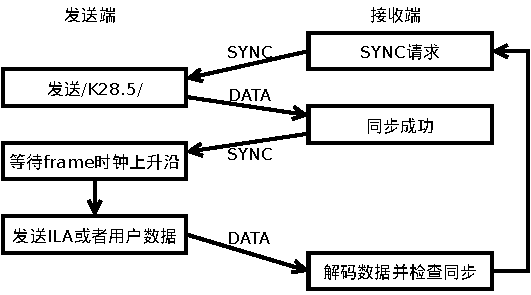
\includegraphics[width=10cm]{./img/cgs_subclass_0.pdf}
\caption{Subclass 0类设备码群同步过程}
\label{fig:cgs_subclass_0}
\end{figure}

对于Subclass 1类或Subclass 2类设备的具体的握手流程,如图\ref{fig:cgs_subclass_1_2}所示。

\begin{figure}[H]
\centering
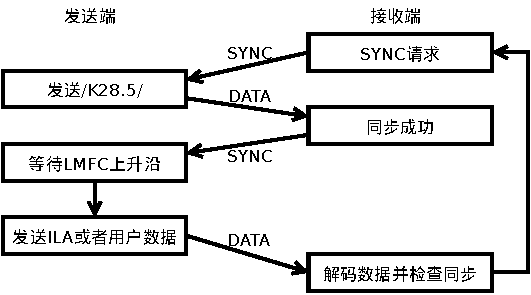
\includegraphics[width=10cm]{./img/cgs_subclass_1_2.pdf}
\caption{Subclass 1类和2类设备码群同步过程}
\label{fig:cgs_subclass_1_2}
\end{figure}

\subsubsection{设计思路}

实际上,码群同步的过程是一直伴随着整个链路的启动过程的,它需要时刻监控链路上的字符信息。
当发送端发送的数据出现连续的错误,或者链路状况变得非常恶劣时,码群同步需要能够检测到这些情况并及时的跳转状态进入到需要重新初始化的状态。
这一过程可以通过一个状态机来描述,如图\ref{fig:cgs_fsm}所示。

\begin{figure}[H]
\centering
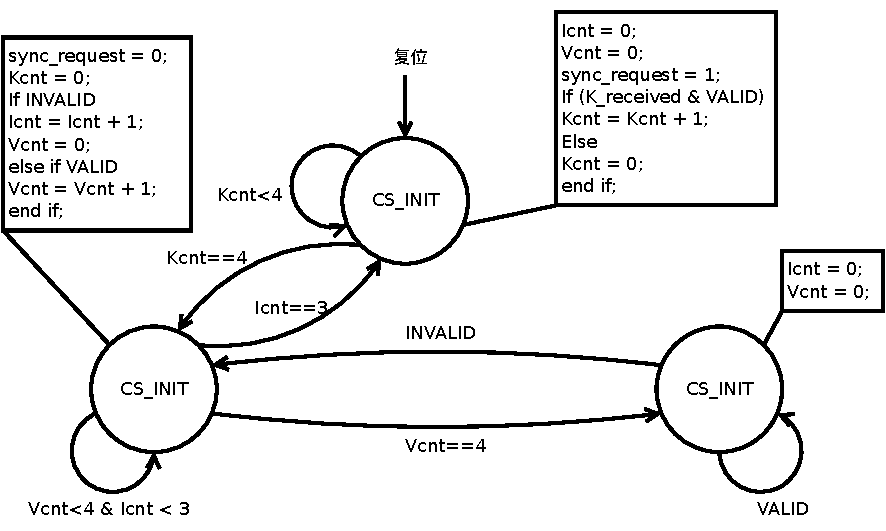
\includegraphics[width=18cm]{./img/cgs_fsm.pdf}
\caption{码群同步有限状态机}
\label{fig:cgs_fsm}
\end{figure}

其中Icnt指的是错误数据的计数,Vcnt指的是正确数据的计数,Kcnt指的是/K28.5/数量的计数,VALID指的是接收到正确的数据,INVALID指的是接收到错误的数据,sync\_request指的是SYNC请求信号。

码群同步在接收端主要有以下几步:
\begin{enumerate}
	\item 当连接启动,接受端发送一个同步请求,发送端传回/K28.5/。
	\item 接收端终止同步条件根据Subclass决定
		\begin{itemize}
			\item Subclass 0:在收到4个连续的/K28.5/后的帧边界终止同步请求。
			\item Subclass 1/2:在收到4个连续的/k28.5/后的本地多帧时钟边界终止同步请求。
		\end{itemize}
	\item 在正确接收另外4个8B/10B字符后,接收端认为码群同步完成。
	\item 当继续收到错误码字后,接收端进入“check”状态。
	\item 如果又有三个错误码字在“check”状态被接收,就表示失去同步。
	\item 如果在“check”状态连续收到4个正常码字,接收端退出“check”状态进入正常运行。
\end{enumerate}

同步请求是通过SYNC接口传送到发送端的。
同步请求被编码成SYNC~信号,保持低电平,并且只可能在接收端frame时钟的上升沿发生变化。
SYNC~信号上最短的同步请求时长是5个frame加9个octets。

接收端只有在激活了同步请求的阶段才允许将/K28.5/作为同步码组。
如果在数据传输阶段,码群码群之间检测到了/K28.5/则视作位错误。

\subsection{初始化帧同步}

当一个link启动时,帧同步的由以下几点实现:

\begin{itemize}
  \item 在码群同步过程中,发送端会一直发送/K28.5/的逗点符号。
  \item 在码群同步结束后,收端会假设收到第一个非/K28.5/符号作为帧的开始。如果发送端开始发送ILAS,那么第一个非/K28.5/字符就是/K28.0/字符。
  \item 接收端假设在每F个octet后就是新的一帧的开始。
\end{itemize}

帧的初始化就是依赖于非/K28.5/字符的开始,并且以配置参数F作为新一帧的界定。
这种以F个octet周期作为一帧的时钟可以作为帧时钟信号,用于界定新的帧,并且能够同步到第一个非/K28.5/符号,以保证帧时钟对齐。
帧时钟是一个很重要的时钟信号,并且在确定性时延中有重要的作用。

\subsubsection{帧对齐和帧纠错}

帧对齐是通过监视帧对齐字符来保证的,这些对齐字符是由发射端在确定情况下加在每一个帧的结尾处。
当接受端收到的错误并不是一个在lane中的位错误时,需要用对齐字符来进行重同步。
通常情况下,只有在相同的位置连续接收到不正确的字符时,才需要进行重同步。
如果是lane对齐导致的帧对齐字符的不正确接收,则不需要在同一位置等待对齐字符。

这里的对齐字符即/K28.7/。
如果两边的lane都支持lane同步,那么lane的对齐字符/K28.3/应该在一个多帧的最后一个帧。
/F/字符即/K28.7/,被编码成0xFC;/A/字符即/K28.3/,被编码成0x7C。
符号替换是否启用,由是否启用扰码和lane同步是否支持替换来决定。
下面就分扰码是否开启来讨论字符的替换问题。

\paragraph{不开启扰码}

如果两边均支持lane同步,那么发送端和接受端中的符号替换在传输层中遵循以下规则:

\begin{itemize}
	\item 当最后的octet在当前帧中并且没有和多帧的结尾发生冲突并且等于前一帧的最后一个octet,那么这个octet将由发送端替换为控制字符/K28.7/。如果前一帧中已经传送了对齐字符,那就发送原数据。
	\item 当现有多帧的最后一个帧的最后一个octet等于前一帧的最后一个octet,发送端需要将这个octet替换成/K28.3/,即使一个控制字符已经在之前发送过了。
	\item 当收到/K28.7/或者/K28.3/时,接收端需要用解码后的数据代替她,或者用上一帧同样位置的数据代替。
\end{itemize}

如果至少有一边不支持lane同步,那么发送端和接受端中的符号替换在传输层中遵循以下规则:

\begin{itemize}
	\item 当现有帧的最后一个octet等于前一帧的最后一个octet,发送端需要用/K28.7/替换这个octet。但是如果在之前的帧已经传输过该控制字,则按原数据发送。
	\item 当收到/K28.7/时,接收端需要用上一帧同样位置的数据代替。
\end{itemize}

\paragraph{开启扰码}

如果两边均支持lane同步,那么发送端和接受端中的符号替换在传输层中遵循以下规则:

\begin{itemize}
	\item 当一个加扰过后的octet位于一个帧的最后位置等于0xFC,并且不在多帧的最后,发送端需要将其编码为/K28.7/。
	\item 当一个加扰过后的octet位于一个多帧的最后位置等于0x7C,发送端需要将其编码为/K28.3/。
	\item 当收到/K28.7/或者/K28.3/时,接收端需要对其解扰。
\end{itemize}

如果至少有一边不支持lane同步,那么发送端和接受端中的符号替换在传输层中遵循以下规则:

\begin{itemize}
	\item 当一个加扰过后的octet位于一个帧的最后位置等于0xFC,发送端需要用/K28.7/替换这个octet。
	\item 当收到/K28.7/时,接收端需要将0xFC放入解扰器。
\end{itemize}

\paragraph{帧同步在接收端的纠错}

当纠错启动时,需要执行以下步骤:

\begin{itemize}
	\item 如果连续两次有效的对齐字符在同一位置被检测到,并且不在接收端认为的正确帧结束位置。在两个对齐字符之间也没接收到一个在期望位置的对齐字符,接收端将会重新对齐帧边界到那个收到的对齐字符位置。
	\item 在重新对lane对齐过后,可能会导致帧对齐错误,接收端将会重新对齐帧到第一次接收到对齐字符的位置。
	\item 接收端需要有一个配置去取消重同步,因为如果没有进行加扰,确定类型的周期信号可能无法产生足够的对齐字符可以用来侦测对齐的失败与否。
\end{itemize}

\subsubsection{设计思路}

根据协议建议,帧同步的过程可以通过有限状态机实现,可以分为两种情况。
一是需要支持数据接口重同步请求的设备中,另一种是不需要支持重同步请求的设备。
第一种设备的有限状态机设计如图\ref{fig:ifs_fsm_resync}所示,第二种设备的有限状态机设计如图\ref{fig:ifs_fsm_non_resync}所示。

图\ref{fig:ifs_fsm_resync}所示是带重同步功能的初始化帧同步的有限状态机描述。
\begin{figure}[H]
	\centering
	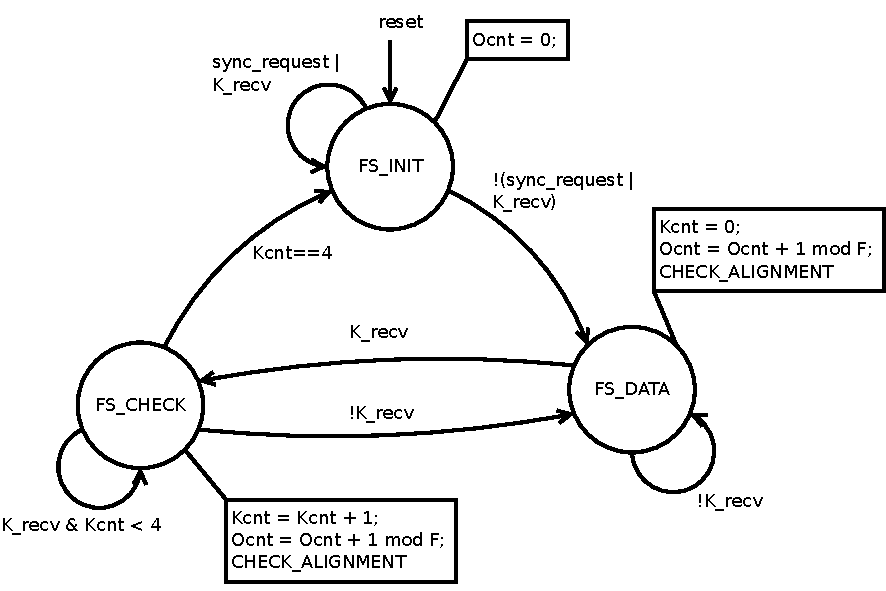
\includegraphics[width=16cm]{./img/ifs_fsm_resync.pdf}
	\caption{有重同步的初始化帧同步有限状态机}
	\label{fig:ifs_fsm_resync}
\end{figure}

图\ref{fig:ifs_fsm_non_resync}所示是不带重同步功能的初始化帧同步的有限状态机描述。
\begin{figure}[H]
	\centering
	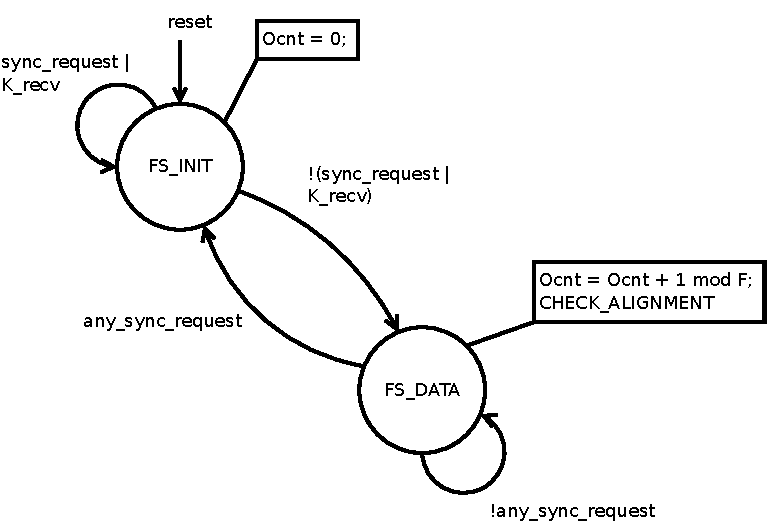
\includegraphics[width=16cm]{./img/ifs_fsm_non_resync.pdf}
	\caption{没有重同步初始化帧同步有限状态机}
	\label{fig:ifs_fsm_non_resync}
\end{figure}

其中,any\_sync\_request指的是任意连接在link上的接收端的同步请求;CHECK\_ALIGNMENT指的是对帧对齐监控;K\_recv指的是标示现在收到的符号为/K28.5/;Kcnt指的是在FS\_CHECK状态对有效的/K28.5/计数;sync\_request指的是接收端检测到失去码群同步,发出同步请求,或者发生别的错误需要重初始化;F指的是每个帧的octet数;Ocnt指的是标记此帧中的当前octet位置。

在设备重置后,状态机进入初始化状态,octet计数器被清零,码群同步激活,接收端启动同步请求。
同步请求的激活状态会使帧同步保持在初始化状态。
当同步请求被取消后,状态机转入FS\_DATA状态,同时发射端停止发送/K28.5/符号。
在FS\_DATA状态,octet计数器Ocnt统计该帧中的octet数目,在0和F-1之间。
如果link中任何一个接收端启动了同步请求,就要从FS\_DATA状态进入FS\_INIT状态。
这种情况只会发生在监视器检测接收到了/K28.5/,在多接收端的设备中。

如果/K28.5/被接收到,状态机进入FS\_CHECK状态,在这个状态octet计数器Ocnt继续工作。
如果连续4个/K28.5/被接收到,帧同步回到FS\_INIT状态。
对于只配置成单接收端的设备,可以监测到所有接收端各自的同步请求。

同样的,对于重对齐的检测和纠错,协议也给出了建议。
监测和纠错的过程由以下伪代码所示。
纠错功能应该可以通过寄存器设置来关闭或者开启(RESET\_OCTET\_COUNTER),尤其是当用户数据不能产生有效的对齐字符以供监测的时候。

\begin{algorithm}[H]
	\caption{帧对齐监测和纠错}
    \begin{algorithmic}[1]
    	\If{(A\_recv | F\_recv)}
    		\State REPLACE\_ALIGNMENT\_CHARACTER;
    		\If{(((Ocnt == previous\_AF\_position) | CROSS\_COUPLING) \& VALID)}
    			\State RESET\_OCTET\_COUNTER;
    		\EndIf
    		\If{VALID | (Ocnt == F-1)}
    			\State previous\_AF\_position = Ocnt;
    		\EndIf
    	\EndIf
    \end{algorithmic}
\end{algorithm}

其中,A\_recv表示接收到了/K28.3/,即/A/字符;CROSS\_COUPLING指的是由于lane和帧之间的对齐交叉配对导致帧失去同步;F指的是每个帧的octet数;F\_recv表示接收到了/K28.7/;Ocnt表示此帧中的当前octet位置;previous\_AF\_position记录/K28.3/或/K28.7/在帧中的位置;RESET\_OCTET\_COUNTER指在接收到下一个octet时,重置octet计数至0;VALID表示在给定极性情况下收到的正确码字。

REPLACE\_ALIGNMENT\_CHARACTER用以下字符替换在解码输出处的对齐字符:
\begin{itemize}
	\item 当扰码取消时,用上一帧同样位置的数据,或者实用解码后的数据;
	\item 当扰码启用时,数据字符保持不变。
\end{itemize}
记录下/K28.3/的位置,如果在lane同步或者lane对齐监测中需要。

\subsection{初始化lane同步}

\subsubsection{协议分析}

在具体数据发送之前需要进行初始化lane同步。
lane同步使用具体的控制字/K28.3/。
对于发送端来说,会在一个固定的时间点,所有的lane同时发送lane对齐字符/K28.3/。
对于不同的lane会产生不同的延时,不同lane的对齐字符可能在不同时刻被接收到。
每个接收端在收到/K28.3/后,会对对收到的数据进行缓存,并且对别的接受端标志出“ready”状态,表示缓存里已经有了一个有效的对齐起点。
当所有的接收端标示了对齐接收到的标志后,会在规定的同一个时刻传输接收到的数据,以保证数据的同步。

对于JESD204B设备,支持确定时延,所以具体的开始数据传输时刻会有具体的规定,将在确定性时延章节具体讨论。
确定性时延能够设置一段时间的延时用来保证所有的lane收到对齐字符。

初始化lane同步在码群同步结束后立即开始执行,依靠的是发送ILAS。
不需要对ILAS进行加扰。
作为模数转换器设备会固定的传输4个多帧的ILAS,对于Subclass 1和2的数模转换设备会固定接收4个多帧的ILAS。
同时配置多个Subclass 0类的数模转换器设备可能需要更多多帧的ILAS来保证lane的对齐。
而对于逻辑设备来说,ILAS需要能够设置成4到256个多帧的长度。
这里一个多帧就指的是K个连续的帧,这里的K值是介于1和32之间的数,即表示每个多帧的octet数是介于17和1024之间的值。

具体K的范围如下式所示:

$$ceil(17/F) \le K \le min(32, floor(1024/F))$$

对于JESD204发送设备来说,K的值应该是可编程的。
对于JESD204接收设备来说,K的值也建议设置成可编程。
与此同时,接收设备也要给出建议的K配置值,方便发送设备配置具体的数值。

\begin{figure}[H]
	\centering
	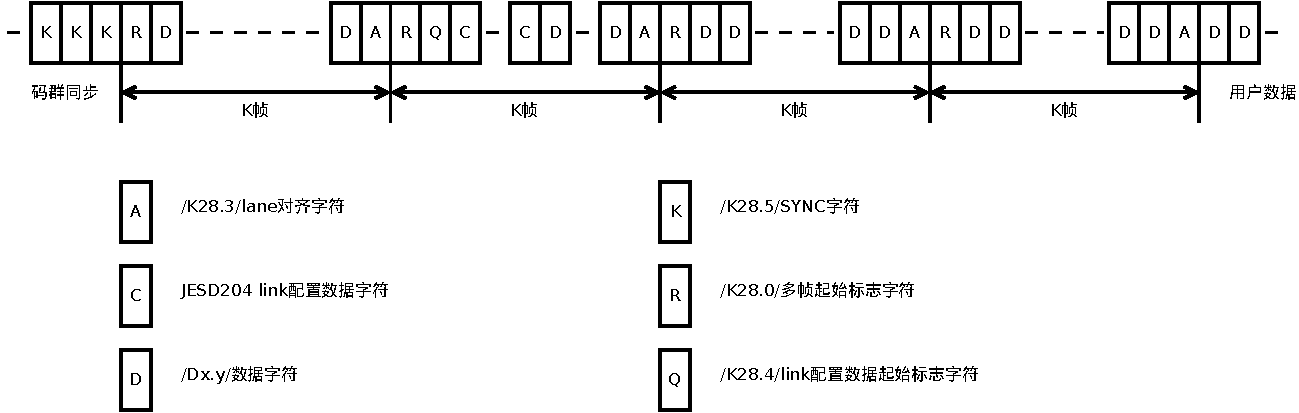
\includegraphics[width=16cm]{./img/ilas.pdf}
	\caption{ILAS}
	\label{fig:ilas}
\end{figure}

ILAS的结构如图\ref{fig:ilas}所示。
每一个多帧由/K28.0/作为起始,/K28.3/作为结束。
/K28.0/告诉了接收端这个多帧是ILAS的一部分。
/K28.3/作为多帧的结尾,也同时作用于lane和帧同步。
第二个多帧需要包含设置信息,用来配置接收端和发送端的link,从第三个字符开始。
第二个多帧的第二个字符则为/K28.4/,作为再次确认信息,标示之后的数据作为设置参数。

在初始化帧和lane对齐后,信道转换到对齐监视模式。
lane对齐通过观察/K28.3/来实现。
因为/K28.3/是由发射端在确定情况下插入在多帧结尾的控制字。
通常情况下不是所有的lane会同时传送/K28.3/。
每一个接收端可以分别检查所收到的/K28.3/,并同各自的本地时钟比较,以确定是否需要纠正对齐错误。


每个多lane环境下的接收端可以通过更高层的应用确认是否进行重对齐,当以下三种情况同时发生:
\begin{itemize}
	\item 准确的检测到了失去对齐,并且
	\item 发现了一个可靠的新的对齐位置,并且
	\item 在现有缓存中的数据能够实现重对齐。
\end{itemize}
重对齐命令通过接收端的控制接口由更高的层级授权。
lane的重对齐类似于前面提到的帧重对齐。
\begin{itemize}
	\item 如果连续两次有效的对齐字符在同一位置被检测到,并且不在正确的帧结束的位置,而且在两个对齐字符之间也没接收到一个对齐字符,在期望的位置,接收端将会重新对齐帧在那个收到对齐字符的位置。
	\item 在重新对lane对齐过后,可能会导致帧对齐错误,接收端将会重新对齐帧到第一次接收到对齐字符的位置。
\end{itemize}

这里要注意的是,只有当本地的时钟参考是正确时,动态的重对齐能够正确的恢复出lane的时延。
如果lane失去对齐是因为本地时钟参考的相位发生了改变,那么动态的重对齐最终会将所有的lane对齐到相同的参考上,不过link的所有延时都会改变。
为了避免可能的延时改变,Subclass 1类和2类的接收端能够通过SYSREF或者SYNC~信号将本地多帧时钟重新对齐,来实现动态的重对齐。
所有Subclass的接收设备也可以通过发起一个重同步请求来实现动态的重对齐。

在确定错误产生的情况下,接收端能够请求重新初始化link,通过重启一个同步请求。
如果所有的接收端在同一个设备中,所有的同步请求能够被所有的接收端检测到。
这种方式的设备内部同步请求能够对同一设备的所有接收端的帧和lane的同步重新初始化。

另一个方法是通过发送端重置接收端。
因为所有接收端的同步请求被整合到一个SYNC~信号中,这样是同时对所有发送端的同步请求,所有的发送端都会重新发送/K28.5/对任何接收端。
发送端能够通过转换状态到SYNC模式请求重初始化,发送一系列的/K28.5/。

在单独一个设备中的接受端,应该能在4个ILAS多帧的时间内完成相互的lane对齐。
Subclass 1类或者2类设备应该能根据在4个多帧内,对齐新来的对齐字符到内部的本地多帧时钟边界。
当接收端被分成多个Subclass 0类设备,需要设置指定数量的ILAS多帧来完成对齐,但不超过256个多帧。

在设置了多帧的情况下,当任何一个在同一link上的接收端发起了对齐请求,每个接收端都要准备一个新的初始化lane同步。
在设置了单接收端设备时,需要监控所有接收端的设备的同步请求。

\subsubsection{设计思路}

实际上的初始化lane对齐就是对ILAS序列的检测、分析工作和lane的监测工作。
在完成了初始化帧同步后紧接着的就是初始化lane对齐的工作。
当初始化lane对齐完成后就需要对lane进行监控,判断是否需要重对齐。

\paragraph{ILAS序列的检测}

对于接收设备来说,ILAS的长度是数量固定的4个多帧长度,其中的第二个多帧包含了关键的link配置信息。
接收端首先要做的是将4个多帧长度的ILAS拆解,一是提取出对齐信息,一是提取出link配置信息。
比较关键的是对link配置信息的分析,里面主要包含了发送端的一些重要参数。
这些参数会以数据的形式存放,并且确定的位于ILAS多帧中的第二个多帧,紧跟在/K28.4/字符之后。
配置数据的长度为固定的14个octet长度。

其具体组成的块状结构如图\ref{fig:mapping_link_configuration_fields}所示。

\begin{figure}[H]
	\centering
	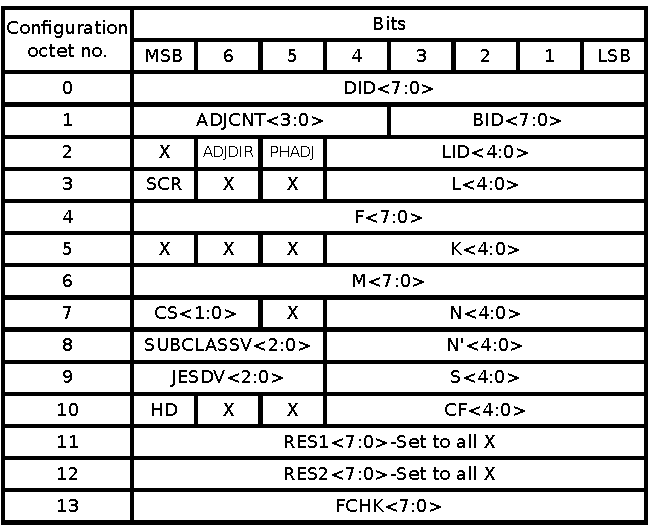
\includegraphics[width=16cm]{./img/mapping_link_configuration_fields.pdf}
	\caption{link配置信息映射图}
	\label{fig:mapping_link_configuration_fields}
\end{figure}

几个主要的具体参数如下所示:

\begin{description}
  \item[ADJCNT] 调整幅度计数,主要是在Subclass 2类设备中用于标识本地多帧时钟的调整数量。
  \item[ADJDIR] 调整方向,主要是在Subclass 2类设备中用于标识本地多帧时钟的调整方向。
  \item[PHADJ] 调整使能,主要是在Subclass 2类设备中用于标识是否调整本地多帧时钟。
  \item[JESDV] 标识JESD版本信息,000为JESD204A,001为JEAD204B。
  \item[SCR] 加扰使能,标识之后的用户数据是否加扰。
  \item[CHKSUM] 校验和,之前数据的和模256。
\end{description}

其余如CS、CF等参数在本章节前面内容有具体介绍,故不再追赘述。

\paragraph{lane对齐监测和纠错}

监测和纠错的过程由以下伪代码所示。
lane对齐监控和纠错通帧对齐监测和纠错非常的相似。
但是它包含了一个额外的步骤,当对齐字符没有到达正确的位置,他会建议在LMFC之间初始化一个同步检测。
当发送端无法发送有效的对齐字符时,lane对齐检查应该可以通过设置来取消。

\begin{algorithm}[H]
	\caption{lane对齐监测和纠错}
    \begin{algorithmic}[1]
    	\If{A\_recv}
    		\State REPLACE\_A;
    		\If{(((Fcnt == previous\_A\_position) | CROSS\_COUPLING) \& VALID)}
    			\State RESET\_FRAME\_COUNTER;
    			\If{(Fcnt != K-1)}
    				\State INITIATE\_SYNC\_CHECK;
    			\EndIf
    		\EndIf
    		\If{VALID | (Fcnt == F-1)}
    			\State previous\_A\_position = Fcnt;
    		\EndIf
    	\EndIf
    \end{algorithmic}
\end{algorithm}

A\_recv表示接收到了/K28.3/;CROSS\_COUPLING指由于lane和帧之间的对齐交叉配对导致帧失去同步;Fcnt表示此多帧中的当前帧位置;K表示单个多帧中帧的数量;previous\_A\_position记录/K28.3/在多帧中的帧位置;RESET\_FRAME\_COUNTER指在接收到下一个帧时,重置帧计数至0;INITIATE\_SYNC\_CHECK指如果通过控制接口,授权被允许,就需要在本地多帧时钟之间初始化一个同步检查;VALID表示在给定极性情况下收到的正确码字。

REPLACE\_A指用以下字符替换在解码输出处的/K28.3/:
\begin{itemize}
	\item 当扰码取消时,用上一帧同样位置的数据,或者实用解码后的数据;
	\item 当扰码启用时,用/D28.3/。
\end{itemize}
如果在帧对齐监测中需要,不替换/K28.3/或者记录下它的位置。

\subsection{SYSREF信号相位检测及时钟生成}

\subsubsection{协议分析}

SYSREF信号是Subclass 1类设备确定性时延的同步对齐边沿。
所有系统中的JESD204B设备通过SYSREF信号保证各个链路之间的同步。
由于SYSREF信号是由外部功能芯片提供的对齐信号,所以需要由接收端主动接收这一个信号并进行同步。
目的是把本地多帧时钟同步到这一对齐边沿上。

接收端对SYSREF信号的同步也并不是完全依照接收到的信号为标准的。
可以通过设置一个容错的门限,以设备时钟数为基准,对SYSREF信号进行采样并和本地多帧时钟对比。
如果误差范围超过了寄存器配置的门限要求,就认为同步出现了比较大的问题,可以有选择的进行同步。

这一模块实际上还负责根据配置产生一系列时钟信号和触发信号,以供之后的模块使用,包括弹性缓冲的释放信号。
弹性缓冲是为了保证确定性时延而设计的缓冲区,用来缓存一些先到的相关数据,以便在确定的时机释放里面的内容,保证信号的同步。
弹性缓冲释放的时机是为了保证所有link间信号的同步。
这一时机的选择非常的重要,在协议中是以本地多帧时钟为基准,并在延后可配置个帧周期后的一个时间点作为缓冲的释放时机。
并且释放的前提是缓冲中已经存在了具体的,能够表示同步的信息字符,比如ILAS的/R/字符。
释放的位置也是以非/K/字符开始,以保证数据对齐。

但是在时机情况下,link间的时延有可能会超过一个本地多帧时钟的长度,而协议规定最大的释放时机时延就是一个本地多帧时钟的长度。
于是在设计中考虑了两段时延以保证在时延不理想的情况下也能很好的完成时钟的同步。
分析时延的特性可以发现,接收端和发送端的芯片在数据传输到具体链路上的具体时延和电路之间传输的具体时延是一个确定的范围。
时延可以分成确定的一部分和不确定的部分,其中确定的部分表示在具体情况下并不会缩短的部分,是电路和传输路径决定的。
而不确定的部分可以是一个范围,也就是说实际上时延的不确定性来自于这一范围,所以真正需要缓冲的是这一端可长可短的不确定时延范围。
设计中考虑了这一特点,所以采取了总时延可以确定的一部分采用帧时钟为单位作为寄存器配置信息,来对本地多帧时钟进行延时。
而不确定部分采取其最大值以处理时钟为单位作为寄存器配置星系,来对时延后的本地多帧时钟再次时延,产生释放缓冲的信号。

另外,协议中提供三种SYSREF信号的同步模式,分别是单次同步(One Shot Sync)、连续同步(Continuous Sync)和单次同步并保持监控(One Shot then Monitor Sync)。

\paragraph{单次同步}

在单次同步模式下,在同步配置完成并被启动后,第一个检测到的SYSREF相位就将作为本地多帧时钟的对齐边沿。
当SYSREF信号和本地多帧时钟的相位差超过了容错范围后,将会启动一个相位调整。
整个LMFC的同步操作只会发生这一次,而SYSREF信号可以一直保持发送的状态。

\paragraph{连续同步}

连续同步模式只会使用在能够提供周期性SYSREF信号的Subclass 1类设备中。
在连续模式中,相位的检测和对齐发生在每一个对齐边沿上。

连续模式和单次模式的区别主要体现在两个方面。
第一是不需要SPI周期来保证装备到设备上,连续模式的每次边沿对齐都是在每个相位检测后。
第二是相位检测发生在每一个对齐边沿。
在相位调整阶段,之后到来的对齐边沿都会被忽略。

容错窗口的大小指的是本地多帧时钟边界和对齐边沿之间存在的最大差错大小。
在连续同步模式下,这个范围不能为零。

\paragraph{单次同步并保持监控}

在这一模式下是,用户能够实时的检测到相位的错误。
使用这种同步模式,需要提供一个周期性的SYSREF信号。
它的单次同步操作和之前描述的单次同步操作类似。
只是在之后的对齐边上,相位始终被监测和报告。
能够通过寄存器数据读出对齐情况。

\subsubsection{设计思路}

本模块的主要作用就是提供几个主要的时钟、触发信号给之后的模块,要求就是尽量保证时钟的准确性。
首先是几个主要的信号。
SYSREF信号就是由时钟芯片产生的主要参考脉冲信号,本地多帧时钟需要对齐到该信号,以保证各个设备间多帧时序的同步。
设备时钟信号推荐的配置也是由产生SYSREF信号的同一时钟芯片产生的主要设备时钟,由同一设备产生最大的好处就是可以尽可能的避免相位之间的区别。
设备时钟信号是内部时钟产生的主要时钟源,需要根据配置能够产生本地多帧时钟信号、帧时钟信号、处理时钟信号等。
帧时钟信号是帧时钟信号,需要根据具体的配置信息F和设备时钟的频率来产生一个帧时序信号用来作为帧的定界。
它是由设备时钟产生的时钟,并且能够在需要的时候对齐到SYSREF信号。
处理时钟信号是4字节处理触发脉冲,设备的数据链路层处理设计的是4字节一组的方式,即表示一次性需要处理4字节的数据,驱动数据处理的节拍就是处理时钟,它的周期就是4/F个帧时钟周期的长度。
最后是本地多帧时钟,这一信号的产生非常重要,它是需要对齐到SYSREF信号的主要时钟。
多帧的配置信息K,表示的是一个多帧内包含的帧的数目。
在整体设计中本模块主要负责处理时钟,提供了SYSREF信号,所以几个重要的时钟信号也是由此模块产生的,包括帧时钟、本地多帧时钟。

为了实现确定性时延,设计首先采取的是通过SYSREF信号同步全局的本地多帧时钟,因此产生出来的本地多帧时钟默认就是对所有设备都是同步的。
再就是lane中先到数据的缓存,通过弹性缓存来保证数据的同步。
实际上的设备间时延可以分作三部分,发送时延、接收时延和传输路径上的时延,其中传输路径上的时延可以认为就是PCB布线长度的时延,这部分是可以精确计算的。
对于发送时延和接收时延可以分为两部分,一部分是确定的时延,一部分是不确定的时延。
所谓确定的时延就是发送和接收过程中,同步数据在芯片内部传递经过的具体时延,这一部分在芯片设计过程中是可以确定的。
比如说8B/10B的解码需要一个处理时钟周期的时间,这就是确定的时延的一部分。
而不确定的部分就是可能产生的一些不确定的情况引起的时延变化,比如一个组合逻辑在不同的情况下可能会产生不同的时延,又比如对齐时钟沿的不确定性,这些不确定性就决定了时延的不确定部分。
但是不确定部分是有一个具体的范围的,由精度能够得出一个大致的范围,例如正负20纳秒这样的不确定范围。

由此可以将设备的时延又细分为两部分,一部分是确定的,一部分是不确定的。
这两部分的具体数据是可以计算出来的,并且需要作为芯片特性的一部分载入手册以供设计时参考,均以纳秒为单位。
时延的确定部分其实对于所有lane来说都是一样的,也就是任何信号从发端发出到收端收到都无法避免的必须经过这一确定的过程。
数据到达接收端的先后顺序主要是由不确定部分决定的,不确定部分相当于传输数据的一个窗口,表示各个lane之间可能会在这个窗口中产生相位的不同步。
实际上这一部分是相对较小的,也是实际上真正需要接收端缓冲的部分。
接收端对于确定的部分采用的办法是直接将本地多帧时钟延时LMFCDEL个帧时钟周期,产生LMFC\_RX信号,解决了时延中共性的部分。
然后芯片又对于不确定的部分采取将LMFC\_RX信号延时LMFCVAR个处理时钟周期的方法产生了一个缓冲释放的信号,来作为收端同步的信号。
而收端缓冲的大小设计成10个处理时钟周期的大小,即为40字节每个lane,也就是说芯片能够接受的最大不确定性是10个处理时钟周期的范围。
如果最晚到达和最早到达相差超过10个处理时钟周期,则很有可能出现无法对齐的情况。
而释放这个缓冲的时机是根据时延的不确定性部分计算出来的,以处理时钟周期的形式表示,作为配置信息的一部分。

以上分析的是芯片提供了具体可参考的时延信息。
如果面对陌生的芯片,无法准确的计算出时延不确定的部分和确定部分的值。
这种陌生的情况下,设备通过设计一个时延的计数器,通过实际的传输统计link间时延的差别,计算得到具体情况下的时延配置参数。
这种时延差别的计数是以处理时钟为单位,具体指的就是本地多帧时钟边界和第一个收到数据字符之间的相位差。
通过配置寄存器的读写,能够在这个模块中读出具体时延,经过反复试验,计算最合适的配置值。
最终还是通过配置寄存器的方式完成link的配置,保证时延的确定性。

\bibliography{../../bib/serdes}
\end{document}
